% !TEX ecnoding = UTF-8 Unicode

\documentclass[a4paper]{article}

\usepackage{color}
\usepackage{url}
\usepackage[T1]{fontenc}
\usepackage[utf8]{inputenc}
\usepackage{graphicx}
\usepackage{caption}
\usepackage{colortbl}

\graphicspath{ {images/} }
\usepackage{listings}
\usepackage{xcolor}

\usepackage{dirtytalk}

\newtheorem{primer}{Primer}[section]

\usepackage[english,serbian]{babel}

\usepackage[unicode]{hyperref}
\hypersetup{colorlinks, citecolor=green,filecolor=green,linkcolor=blue,urlcolor=blue}

\begin{document}

\title{\vspace{-5ex}Propusti u bezbednosti veb aplikacija i prevencija njihove zloupotrebe\\ \small{Seminarski rad u okviru kursa\\Metodologija stručnog i naučnog rada\\ Matematički fakultet}}

\author{Aleksandra Kovačević, David Ivić, Sreten Kovačević\\ mi13302@matf.bg.ac.rs, 310ddavi@gmail.com, mi13097@matf.bg.ac.rs}

\maketitle

\abstract{Ovaj rad pruža osnovne informacije o bezbednosti softvera, posledicama koje nastaju usled njenog zanemarivanja i načinima prevencije njenih zloupotreba. Akcenat će biti na bezbednosti veb aplikacija. Takođe, prikazana je i potreba za adekvatnom bezbednošću celog sistema, a ne samo aplikacija. Kroz primere su, na praktičan način, prikazani razlozi i preporuke za implementaciju bezbednog softvera.}

\tableofcontents

\newpage

\section{Uvod}

Propusti u bezbednosti softvera mogu biti vrlo problematični za informacione sisteme, pogotovu one u komercijalnoj primeni, koji rade sa velikom količinom poverljivih podataka, te je ovo tema koja je vrlo zastupljena u modernom računarstvu. Kako se količina podataka povećava velikom brzinom i sve je veći broj aplikacija koje rade na vebu, očekuje se da značaj ovog problema postaje sve bitniji.

U okviru ovog rada ćemo se susresti sa osnovnim pojmovima i konceptima ovog problema. U odeljku \ref{bezbednost}, koji se tiče bezbednosti softvera, upoznaćemo se sa nekim principima koji se koriste sa ciljem implementacije softvera sa minimalnim brojem bezbednosnih rizika \cite{BIS}. Nakon upoznavanja sa osnovama bezbednosti, u odeljku \ref{aplikacije}, imaćemo priliku da se upoznamo sa nekim od čestih tipova napada na veb aplikacije \cite{SQL, XSS, AC}, kao i načinima za njihovu prevenciju. Kroz primere \ref{primer2}, \ref{primer3} i \ref{primer4}, videćemo pojednostavljene verzije ovih napada na delu.

Prelaskom na odeljak \ref{server}, sa problema bezbednosti aplikacija preći ćemo i na problem bezbednosti okruženja na kom se aplikacija izvršava. Dotaći ćemo se i smernica za pravilno održavanja servera \cite{WS}. U zaklju\v{c}ku \ref{zakljucak} je dat kratak pregled najbitnijih stavki koje su obrađene u ovom radu, kao i dodatne smernice za dalji nastavak istraživačkog rada. Osim toga, ukratko je opisan i problem koji nastaje ukoliko prevencija zakaže.

\section{Bezbednost softvera} \label{bezbednost}

Bezbednost softvera je ideja pri konstruisanju softvera, koja podrazumeva da on nastavi da funkcioniše ispravno čak i u specijalnim situacijama. Specijalne situacije mogu se odnositi kako na zlonamerne napade, tako i na nepravilno korišćenje aplikacije od strane nestručnog korisnika.

Najbolja praksa pri razvoju bezbednog softvera uključuje razmišljanje o sigurnosti u ranim fazama životnog ciklusa softvera, razumevajući uobičajene pretnje (uključujući i mane programskog jezika), podvrgavajući sve softverske nepravilnosti temeljnoj i objektivnoj analizi rizika i testiranju. Dok softveri koji se razvijaju uglavnom imaju greške pri implementaciji, utvrđeno je da je sigurnost mnogih sistema narušena zbog mana u dizajnu softverskog rešenja.

U nastavku ćemo govoriti o osnovnim principima dizajna bezbednog softvera. Kako je ova oblast prilično široka, pomenućemo samo one najvažnije. Fokus će biti na veb aplikacijama. Bitno je napomenuti da neće biti reči o operativnim sistemima, antivirusnoj zaštiti i zaštitnom zidu, koji su bitni aspekti bezbednosti sistema, ali nisu direktno vezani za dizajn softvera.

\subsection{Kontrola pristupa podacima}
Jedan od ciljeva sigurnosnog dizajna softvera je da se spreči entitet (korisnik ili napadač) od neovlašćenog pristupa sistemu. Pristup zaštićenim informacijama mora biti ograničen na lica koja imaju prava pristupa takvim informacijama, u suprotnom može doći do neautorizovanog pristupa, upotrebe, menjanja, uništavanja kao i sprečavanja raspoloživosti.

Osnovni predmeti ugrožavanja su poverljivost (sposobnost da se sopstveni podaci zaštite od neovlašćenog pristupa), integritet (sposobnost da se spreči neovlašćeno ili nepoželjno menjanje podataka) i raspoloživost informacija (sposobnost da se pristupa podacima kada su potrebni).\cite{BIS}

Kontrola pristupa se ostvaruje u tri koraka:
\begin{itemize}
	\item Identifikacija
	\item Autentikacija
	\item Autorizacija
\end{itemize}
Na slici \ref{slika1} možemo videti redosled primene koraka kontrole pristupa prilikom pristupanja osetljivom resursu.

\begin{figure}[h]
\begin{center}
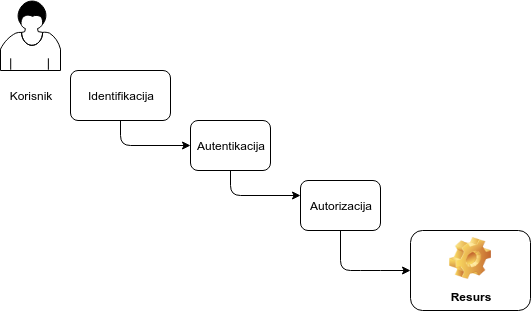
\includegraphics[scale=0.4]{koraci}
\caption{Koraci prilikom pristupanja osetljivom resursu}
\label{slika1}
\end{center}
\end{figure}

\subsubsection{Identifikacija}
Identifikacija je pretpostavljanje identiteta subjekta. Uobičajeno se odvija na osnovu korisničkog imena, broja računa, ID kartice. Uglavnom nije jedinstvena i sama za sebe predstavlja veoma slab koncept.

\subsubsection{Autentikacija}
Autentikacija je skup metoda za ustanovljavanje istinitosti saopštenog identiteta. Faktori autentikacije su elementi koji učestvuju u proveri (što je više faktora to je tehnika pouzdanija).

Tehnike autentikacije: 
    \begin{itemize}
        \item Memorijski faktori (lozinka, PIN)
        \item  Biometrijski faktori (visina, težina, otisak prsta, rukopis)
        \item Fizički faktori (ID kartica, token)
        \item Logički (neka pravila reagovanja na različite uslove)                                    
        \item Geografski (Lokacija korisnika)                                
    \end{itemize}

Daleko najpopularniji mehanizam za autentikaciju ostaje lozinka. Korišćenje lozinke zahteva da sistem ili servis 
ima mehanizam koji povezuje datu lozinku sa konkretnim korisnikom. Ako ova informacija nije sačuvana na dobar 
način, postoji mogućnost da će neko drugi sem korisnika dobiti pristup njoj.

Nakon uspešne autentikacije, korisniku mora biti 
dodeljen kredencijal autentikacije ili token, tako da korisnik 
ne mora da se ponovo autentikuje svaki put kada hoće da izvrši novi zahtev ili transakciju na sistemu. 
Istovremeno, ako je napadač u mogućnosti da falsifikuje ove kredencijale ili token, on može lako zaobići 
mehanizam autentikacije. Jedan od načina zaštite protiv falsifikovanja kredencijala je korišćenje 
kriptografskih algoritama pri pravljenju kredencijala ili tokena.\cite{Top10}

Sistem za autentikaciju treba da bude dizajniran tako da automatski zahteva ponovnu autentikaciju nakon nekog 
perioda neaktivnosti ili pre neke kritične operacije.
Ako sistem za autentikaciju ne ograniči vremenski period za koji će korisnik biti autentikovan onda može 
da dopusti pristup korisnicima kojima ne bi trebalo. Zamislimo korisnika koji se prijavljuje na javni terminal
i onda odlazi, pritom zaboravljajući da se odjavi. Ispravno dizajniran sistem za autentikaciju 
će automatski odjaviti korisnika, nakon nekog perioda neaktivnosti.

\subsubsection{Autorizacija}
Autorizacija predstavlja mehanizam provere prava specifičnog subjekta.
Samo znanje korisnikovog identiteta može biti nedovoljno za izvršavanje određene operacije, već je neophodno znati koje su njegove privilegije.
Na primer, kada ATM (eng.~{\em Automated Teller Machine}\footnote{Bankomat}) mašina autentikuje korisnika putem fizičkog faktora (bankovna kartica) i memorijskog faktora (PIN kod),
to ne znači da je tom korisniku dozvoljeno da podigne proizvoljnu sumu novca sa svog računa. Većina korisnika je autorizovana 
da podigne sumu novca do neke određene dnevne granice, ili da izvršava neke određene operacije (upit stanja), 
ali ne i druge (prenos novca van banke) sa ATM-a.
 
Za posebno osetljive operacije, autorizacija možda mora da se ponovo obrati autentikaciji, iako autorizacija počinje tek 
nakon autentikacije. Autentikacijom od korisnika može biti zahtevano da pruži minimalan ili značajniji dokaz njegovog identiteta. 
Na primer, prenos sume novca veće od dizajniranog praga prenosa može zahtevati ponovnu autentikaciju, ili veći nivo autorizacije.

Neke politike zahtevaju dvoje ljudi da bi se autorizovala kritična transakcija. U tom slučaju 
bitno je da se uveri da su dve osobe različite pa autentikacija putem lozinke nije dovoljna za ovu svrhu.

\subsection{Kriptovanje podataka}
Kriptografija\cite{CRYP} je grana matematike koja se zasniva na zaštiti podataka kroz njihovu transformaciju. Predstavlja veoma bitan alat koji se koristi u mnogim bezbednosnim aspektima. Na primer, primena kriptografije može doprineti obezbeđivanju integriteta i poverljivosti podataka i implementaciji naprednih metoda autentikacije korisnika.

Kriptografija se sastoji iz dve osnovne komponente, algoritma i ključa. U modernim kriptografskim sistemima algoritmi predstavljaju kompleksne matematičke formule, dok su ključevi nizovi bita. Na osnovu kljča i agoritma se  vrši odgovarajuća transformacija nad podacima. Da bi dve strane komunicirale, moraju koristiti isti algoritam (ili algoritme koji su dizajnirani da rade zajedno) i uglavnom isti ključ.

Ovu oblast nećemo detaljnije obrađivati u okiru ovog rada.


\subsection{Eksplicitna provera podataka}
Softverski sistemi i komponente obično prave pretpostavke o podacima nad kojima rade. Veoma je bitno da se eksplicitno obezbedi da te pretpostavke ustvari važe. Ranjivosti sistema su često prouzrokovane iz implicitnih pretpostavki o podacima, koje mogu biti razotkrivene ako napadač zavara ove pretpostavke.
Kao takav, bitno je da dizajn softverskog sistema obezbedi da se validacija podataka zaista izvrši i da su sve 
pretpostavke o podacima potvrđene.\cite{Top10Flaws}

Kako bi se obezbedila kvalitetna validacija podataka, neophodno je koristiti kombinacije sledećih pristupa:
\begin{itemize}
	\item \textit{Centralizovani mehanizam za validaciju} - svi podaci koji ulaze u sistem moraju da prođu kroz osnovne korake validacije pre nego što sistem počne da ih upotrebljava
	\item \textit{Validacija često ponovljenih podataka} - poželjno je koristiti već postojeće biblioteke za provere ispravnosti čestih formata podataka kao što su adrese elektronske pošte
	\item \textit{Upotreba provere tipova na implementacionom nivou jezika} - često možemo iskoristiti svojstva već postojećih tipova u korišćenom programskom jeziku za provere podataka koje koristimo, kao što je format datuma
\end{itemize}
Ukoliko se ne pridržavamo ovih principa može doći do pojave mnogih sigurnosnih rizika, od kojih je jedan ilustrovan u primeru \ref{primer5}

\begin{primer}
	\label{primer5}
	Ukoliko se za implementaciju koristi jezik koji nema automatsku kontrolu memorijskog pristupa, poput C programskog jezika, i ne proveri se ispravnost ulaza, može doći do različitih problema, kao što su prekoračenje bafera, pristupanje memoriji van opsega, neispravne niske... Svaki od ovih problema za uzrok može imati nasilno prekidanje rada programa, što je najpovoljnije u cilju bezbednosti. Na taj način napadač je sprečen da proširuje svoj napad (u slučaju da se program ne prekine, već da se nađe u nekom stanju greške, napadač može zaobići bezbednosne mehanizme, vršiti izmene podataka...).
\end{primer}

\section{Bezbednost veb aplikacija} \label{aplikacije}

Sa pojavom Veb 2.0, povećanjem deljenja informacija preko socijalnih mreža i korišćenjem veba kao sredstva poslovanja i pružanja različitih informacija, bezbednost sajtova često biva ugrožena upadima od strane zlonamernih korisnika.

Zlonamerni korisnici (u daljem tekstu hakeri\footnote{Pojam haker sugeriše na stručnjaka iz oblasti računarskih nauka koji ima kapacitete da rešava probleme sa kojima se suočava. Vremenom, reč haker postala je sinonim za ljude koji koriste nedostatke u programu kako bi upali u računarski sistem.}) ili nastoje da kompromituju korporativnu mrežu ili navode krajnje korisnike koji joj pristupaju ka preuzimanju sadržaja čijeg rizika nisu svesni (zlonamerni programi, odnosno virusi). Kao rezultat toga, industrija obraća veliku pažnju na bezbednost samih veb aplikacija, pored bezbednosti osnovne računarske mreže i operativnih sistema.

Bezbednost veba je grana bezbednosti informacija koja se bavi bezbednošću veb sajtova, veb aplikacija i veb servera. Bezbednost veb aplikacija se oslanja na principe bezbednosti aplikacija uopšte, ali ih primenjuje specifično za Internet i veb sisteme.
Bezbednost veb servera je zaštita informacija dostupnih preko veb servera. Te informacije se mogu ugroziti povećanim sigurnosnim rizicima i propustima prilikom implementacije.

\subsection{Sigurnosni rizici}

Najveći sigurnosni rizici potiču iz nerazumevanja sposobnosti hakera. Kada se razmišlja o zaštiti veb aplikacije, ne sme se voditi mišlju: sve što je prikazano, biva naše ograničenje onoga što možemo da učinimo. Sve što predstavlja klijentsku stranu i ograničenja koja su pomoću nje nametnuta, mogu se veoma lako zaobići.

Pretraživač ne predstavlja ograničenje. Ne smemo se oslanjati na to da korisnik neće sam uneti parametre koje želi, već treba i na nivou aplikacije da ograničimo prava pristupa.

U okrviru ovog rada, razmatraćemo tri najinteresantnije vrste napada iz ugla zloupotrebe propusta u dizajnu aplikacija:
\begin{enumerate}
	\item Umetanje skriptova (eng.~{\em Cross-Site Scripting})
	\item Umetanje SQL upita (eng.~{\em Direct Object References})
	\item Kontrola pristupa (eng.~{\em Access control})
\end{enumerate}
\subsection{Umetanje skriptova (XSS)}
Umetanje skriptova, poznatiji kao XSS \cite{XSS}, je napad umetanjem(eng.~{\em \\injection}) kodova u sajt. Takođe je jedan od najuobičajenijih načina napada, jer većina sajtova zahteva od korisničkog pretraživača podršku Javascript-a.\\
\textbf{Problem:} Korisnik je u situaciji da pošalje neki vid odgovora stranici (npr. polje za pretragu (eng.~{\em searchbox})), a ako taj odgovor sadrži neke HTML tagove ili Javascript kod, stranica ih renderuje i izvršava kod.\\
\textbf{Posledice:}
\begin{enumerate}
	\item krađa ID-a sesije i samim tim krađa korisnikovog identiteta (u cilju obavljanja poslova u ime tog korisnika)
	\item kontrola stranice (blokiranje rada, menjanje pojedinačnih elemenata...)
	\item redirekcija na drugu, zlonamernu stranicu
\end{enumerate}
U nastavku videćemo različite vrste napada tipa XSS.

\subsubsection{Refleksivni XSS}

Refleksivni XSS (eng.~{\em Reflected XSS}) napad se zasniva na umetanju izvršnog koda u HTTP odgovor. Sam kod nije sačuvan u okviru aplikacije, već (u naivnim primerima) može biti vidljiv u okviru nadograđenog URL-a (eng.~{\em Uniform Resource Locator}), kao posledica HTTP odgovora.
\begin{primer}
\label{primer1}
Pretpostavimo da imamo jednostavan sajt, čija je uloga da ima jedno polje za unos i dugme 'pretraga' (sadržaj onoga što pretražujemo nije bitan za ovaj napad)
\begin{enumerate}
\item nakon bilo kakve pretrage, promeniće nam se URL:\\
\texttt{www.sajt.com?key="pretrazujemo"}
\item izmenom sadržaja sekcije 'key', možemo da ubacimo neki skript

\begin{lstlisting}[language=HTML]
<script>alert("123")</script>
\end{lstlisting}

(isti efekat možemo postići i sa unošenjem takvog koda unutar polja za unos i izvršiti pretragu)
\item Unošenjem takvog URL-a u naš pretraživač (ili kliknom na dugme 'pretraga') ispisivaće se poruka \say{123}\\

\end{enumerate}
\end{primer}

 Naravno, primer \ref{primer1} je jednostavan primer bez vidljivih znakova opasnosti, ali na sličnom principu deluju zlonamerni mail-ovi koji nam pristižu ili sajtovi (ili čak korisnici) koji nameću linkove da korisnik klikne na njih.\\
Način prikrivanja ovakvih napada (jer korisnik može da nasluti iz URL-a da je reč o linku ka zlonamernoj strani) jesu aplikacije za skraćivanje URL-a (eng.~{\em URL shortener})\footnote{Skraćivač URL-a se koristi za skraćivanje njegove dužine, izmenjen zapis, a pritom ne menjajući lokaciju (resurs) na koji referiše.}

\subsubsection{Sačuvani XSS}

Suprotno Refleksivnom XSS-u koji ne ostavlja tragove na samoj aplikaciji, odnosno unutar njenog koda je sačuvani XSS (eng.~{\em Stored XSS}).\\ Cilj sačuvanog XSS-a je da sakrije svoju zlonamernost tako što je javan. Najprostiji primer jeste da u okviru napadnute aplikacije, haker ostavi link ka zlonamernoj stranici i čeka se na korisnika (bilo kog koji nailazi na taj sajt) klikne na njega.

\subsubsection{XSS - prevencija}

Sprečavanje XSS \cite{XSS_prev} napada se oslanja na to što pretraživač renderuje HTML tagove i izvršava Javascript kod.  

Rešenje je da pretraživač uradi enkodiranje na izlazu. Svaki karakter se enkoduje kao što je i prikazano na tabeli \ref{kodiranje}.

Rezultat ovoga je prikaz bezopasne renderovane HTML stranice (premda je problem samo premešten sa bezbednosnog na vizuelni).


\begin{table}[ht]

\begin{center}
\caption{Enkodovanje}
\begin{tabular}{ | c | c | }
\hline
	\rowcolor{yellow}
\textbf{ASCII kodovi} & \textbf{enkodovan HTML} \\
	\hline
 < & \&lt; \\ 
 \hline
 > & \&gt; \\  
 \hline
 \& & \&amp \\
 \hline
 Jednostruki navodnici (') & \&\#039;\\
 \hline
 Dvostruki navodnici (") & \&quot;\\  
 \hline  
\end{tabular}

\label{kodiranje}
\end{center}
\end{table}

\subsection{Umetanje SQL upita}

Umetanje SQL upita (eng.~{\em SQL injection}) \cite{SQL} predstavlja još jedan vid napada umetanjem kodova (tačnije upita) u sajt, ali ovaj put, glavna meta je baza podataka koju koristi server.\\
\textbf{Problem:} Podaci se šalju od strane korisnika, a sistem ne rukuje sa njima na pravilan način.\\
\textbf{Posledice:} 
\begin{enumerate}
	\item neovlašćen pristup bazi i njen pregled
	\item modifikovanje baze izvršavanjem upita (brisanje podataka, menjanje...)
\end{enumerate}

\subsubsection{Umetanje SQL upita - primena}

Umetanje SQL upita se može vršiti u bilo kom delu aplikacije koja u pozadini izvršava neki upit (najčešće je to deo za prijavljivanje (eng.~{\em Log In}), pretraga u okviru sajta, učitavanje podataka iz spoljašnjih izvora itd.). U primeru \ref{primer2} možemo videti napad u fazi prijavljivanja korisnika. Ovo je uprošćen primer, ali svi komplikovaniji se zasnivaju na istoj ideji.
\begin{primer}
\label{primer2}
Pretpostavimo da imamo stranicu, koja nakon uspešnog prijavljivanja ispisuje informacije o korisniku (njegovo korisničko ime i lozinku, neke informacije o njemu itd.). Ukoliko su korisnički parametri uneti kao:\\
- IME: \say{Marko}\\
- LOZINKA: \say{passw0rd}\\
Upit nakon uvrštavanja parametara izgleda:

\begin{lstlisting}[language=SQL]
SELECT * 
FROM baza 
WHERE username='Marko' AND password='passw0rd'
\end{lstlisting}
Uneto ime i lozinka predstavljaju parametre za izvršavanje ovog upita.\\\\
Ako bismo u polje za korisničko ime uneli sledeće:\\
- IME: \say{ hi' OR '1'='1 }\\
- LOZINKA: \say{ hi' OR '1'='1 }\\
Upit bi izgledao sada ovako nakon uvrštavanja parametara:

\begin{lstlisting}[language=SQL]
SELECT * 
FROM baza 
WHERE username='hi' OR '1'='1' 
	AND password='hi' OR '1'='1'
\end{lstlisting}

Primetimo da je izraz \say{1=1} uvek tačan pa je deo za korisničko ime i lozinku krajnje irelevantan.\\
Sistem će prijaviti korisnika (najčesće) sa kredencijalima korisnika koji se nalazi na prvom mestu spiska korisnika iz baze.\\
\end{primer}

\subsubsection{Umetanje SQL upita - prevencija}

Rešenje koje se nameće za umetanje SQL upita, jeste da sistem pravilno proverava niske karaktera koji su uneti kao korisničko ime ili lozinka (konkretno u našem primeru). Glavni problem i jeste u korišćenju specijalnih karaktera (kao što su = ili ' itd.) \cite{SQL_prev}, te treba navesti sistem da ih ignoriše.\cite{Sanit}\\
Takođe postoje i softveri namenjeni proveri \say{ranjivosti} veb aplikacije od napada umetanjem, uz predloge dodatne zaštite.

\subsection{Kontrola pristupa}

Kontrola pristupa \cite{AC} predstavlja filtriranje onoga šta korisnik može da vidi ili sa kojim podacima može da radi,  u zavisnosti od toga koja prava poseduje. Cilj hakera je pristupanje, menjanje nečega za šta ne poseduju prava.\\
\textbf{Problem:} Razvijaoci pretpostavljaju da, ako nešto nije vidljivo korisniku, on ne može da mu pristupi.\\
\textbf{Posledica:} Neovlašćen pristup podacima ili funkcionalnostima.

\subsubsection{Kontrola pristupa - primena}

Direktno referisanje objekata (eng.~{\em Direct Object References}) predstavlja osnovni način zloupotrebe prava pristupa i svodi se na direktno menjanje parametara URL-a.
\begin{primer}
\label{primer3}
Pretpostavimo da imamo sajt banke kod koje imamo otvoren račun i nalog na njemu. Nakon uspešnog prijavljivanja, URL u našem pretraživaču izgledaće ovako:

\texttt{http://banka.com/nalog?id=123}\\
Gde je \say{123} naša reprezentacija sajtu banke. Jednostavnom izmenom \say{123} na npr. \say{124} možemo dobiti pregled drugog korisničkog naloga (najopasnija promena bi bila sa \say{123} na \say{1} jer je to najčešće id administratora sa svim pravima pristupa).
\end{primer}

Osim pregledanja tuđeg naloga, moguće je i korišćenje funkcionalnosti za koja nemamo prava, što pokazuje naredni primer.

\begin{primer}
\label{primer4}
Pretpostavimo da imamo još i dugme za izmenu profila. Klikom na njega, URL će izgledati ovako:

\texttt{http://banka.com/nalog?id=123\&{}action=izmeniProfil}\\
Pretpostavimo da ne možemo mi direktno da izbrišemo nalog sa sajta banke (nemamo vidljivo dugme za tu funkcionalnost, već moramo da šaljemo zahtev administratoru da to uradi), možemo da pretpostavimo (nagađamo) da i ostale akcije imaju slične nazive (npr. \say{action=obrisiProfil}) i da im na taj način neovlašćeno pristupimo.\\
\end{primer}
U primerima \ref{primer3} i \ref{primer4} možemo videti dva načina zloupotrebe kontrole pristupa. Njihova primena se može kombinovati za složenije napade.

\subsubsection{Kontrola pristupa - prevencija}

Ključna stvar jeste da se provere pristupa (autorizacija) rade na serveru (izbegavati \say{Bezbednost prema vidljivosti}(eng.~{\em Security through obsc-urity} \cite{AS})). 

Naivni pristup bi bio i da se ta provera dešava pri svakoj akciji koju korisnik želi da izvrši (potvrda korisničkog imena i lozinke za tu akciju i na osnovu toga provera da li korisnik ima prava za tu akciju).

\subsection{Onemogućavanje usluge}
Onemogućavanje usluge (eng.~{\em Denial of Service - DoS)} \cite{DoSM} predstavlja pokušaj da se neki resurs učini neraspoloživim. Cilj ovog napada nije da omogući pristup ili kontrolu nad udaljenim sistemom već da zauzimanjem svih komunikacionih kapaciteta onemoguće pristup sistemu od strane regularnih korisnika.

Napad se ostvaruje zatrpavanjem usluge mnoštvom zahteva. U jednostavnim slučajevima, napad se izvodi sa jednog uređaja, dok u složenijim može biti koordiniran napad sa više njih (eng.~{\em Distributed Denial of Service - DDoS)}.

Prevencija ovog tipa napada se može implementirati na nivou mreže. Na primer, na nivou zaštitnog zida se može blokirati saobraćaj uređaja sa kog se šalju sumnjivi zahtevi. Još jedan vid prevencije bi bilo nadgledanje mreže i vođenje statistike o prosečnom broju pristiglih zahteva i reagovanje u odnosu na nagle promene.

Ipak, u većini slučajeva  na napad je teško reagovati i pored svih vidova prevencije. Često je neophodno isključivanje servera sa mreže i ponovno pokretanje usluga na njemu.

Neki od čestih tipova napada onemogućavanja usluge su: \cite{DoS}
\begin{itemize}
	\item Prekoračenje bafera - hakeri koriste propust u programu zbog kog podaci koji prekoračuju dužinu bafera budu upisani u drugi bafer, što može dovesti do pada sistema;
	\item TCP SYN napad - napdač zatrpava server TCP zahtevima koji ostaju na čekanju, zbog čega se zahtev legitimnih korisnika nikada ne obrađuje...
\end{itemize}

\section{Bezbednost veb servera} \label{server}

U savremeno doba brojni hakerski napadi nam jasno stavljaju do znanja koliko su serveri \say{ranjivi}, kao i koliko je bitna njihova zaštita. Zaštita same veb aplikacije nam neće biti previše korisna ukoliko nam je server nebezbedan.

Stavke koji su bitne za zaštitu veb servera su:
\begin{itemize}
	\item Uklanjanje nepotrebnih servisa
	\item Udaljeni pristup (eng.~{\em Remote Access})
	\item Održavanje korisničkih naloga
	\item Dozvole i privilegije
	\item Nadgledanje servera
	\item Odvajanje aplikacija i skriptova
	\item Razdvajanje razvojnog i test okruženja...
\end{itemize}

Ove mere ne garantuju, ali u velikoj meri doprinose povećanju bezbednosti veb servera i preporučljivo je pridržavati ih se prilikom njegovog održavanja.\\

\textbf{Uklanjanje nepotrebnih servisa} je poželjno jer svaki servis koji se koristi na veb serveru otvara novi priključak (eng.~{\em port}) na njemu. Na taj način se povećava broj slabih tačaka servera, te ga je teže održavati. Takođe, uklanjanjem nepotrebnih servisa možemo dobiti povećanje performansi kod korišćenih servisa.

\textbf{Udaljeni pristup} koriste administratori za održavanje veb servera. Iako je preporučljivo da se održavanja rade lokalno, nekada to nije moguće, te je neophodno imati omogućenu i ovu opciju na veb serveru. Korisno je ovakav pristup serveru ograničiti na samo određene naloge i IP adrese, kako bi se umanjio bezbednosni rizik nastao njegovim omogućavanjem.

\textbf{Održavanje korisničkih naloga}, poput uklanjanja nepotrebnih servisa, umanjuje broj rizičnih tačaka veb servera. Poželjno je ukloniti ili ograničiti privilegije naloga nastalih prilikom konfigurisanja operativnog sistema ili dodatnih aplikacija.

\textbf{Dozvole i privilegije} treba da budu postavljene u skladu sa realnim potrebama korišćenih servisa. Ukoliko privilegije nadmašuju potrebe, zlonameran korisnik to može iskoristiti za neželjene operacije nad informacijama koje se nalaze na serveru.

\textbf{Nadgledanje servera} podrazumeva praćenje izveštaja, kako sistemskih tako i aplikativnih. Na taj način je moguće blagovremeno uočiti neobična ponašanja aplikacija i sprečiti eventualnu zloupotrebu nedostataka, ali i uočiti pokušaje napada.

\textbf{Odvajanje aplikacija i skriptova} od operativnog sistema i drugih sistemskih podataka je vrlo poželjno. Naime, hakeri koji dođu do pristupa korenom direktorijumu često mogu vrlo jednostavno doći i do dovoljno visokih privilegija da slobodno koriste sve funkcije operativnog sistema. Ovim ograničavamo problem nedovoljne bezbednosti aplikacije tako da ne utiče na druge aplikacije smeštene na tom serveru.

\textbf{Razdvajanje razvojnog i javnog okruženja} pruža dodatnu bezbednost ukoliko razvojno okruženje nije javno dostupno. Veb aplikacije u fazi razvoja često imaju mnogo bezbednosnih nedostataka i ukoliko ti nedostaci postanu javni narušava se bezbednost celokupnog servera. Pogotovu ukoliko aplikacija koja se testira radi sa svim privilegijama, što je česta praksa.

\section{Zaključak} \label{zakljucak}

Predstavili smo različite principe i preporuke za pisanje bezbednog softvera i pripremanje okruženja za neometano funkcionisanje aplikacije. Da rezimiramo:
\begin{itemize}
	\item neophodno je voditi računa o kontroli pristupa podacima,
	\item svaki podatak dostupan aplikaciji neophodno je detaljno proveriti i pripremiti za korišćenje,
	\item posebnu pažnju obratiti na podatke dobijene od korisnika,
	\item ništa ne pretpostavljati i sve potvrditi,
	\item mora se obezbediti da mogućnosti korisnika budu jasno i striktno definisane,
	\item ukoliko okruženje u kom se aplikacija izvršava nije bezbedno - nije bezbedna ni aplikacija.
\end{itemize}

Bitno je napomenuti da nijedan softver nikada nije potpuno bezbedan, te se mora unapređivati. Takođe, sve navedeno u prethodnim poglavljima ne garantuje bezbednost, ali u velikoj meri smanjuje rizik od pojavljivanja propusta i predstavlja dobru praksu prilikom izrade softvera.

Treba imati u vidu i da u slučaju da prevencije ne daju željene rezultate i da napad bude uspešan, uglavnom su mogućnosti administratora dosta male. U tim slučajevima je prvi zadatak uočiti napad, što nije uvek tako jednostavno, pogotovu ukoliko je meta napada poverljivost informacija. Tada, glavnu ulogu ima provera sistemskih i aplikativnih izveštaja.

Nakon detekcije napada, ponekad je potrebno server/radnu stanicu isključiti sa mreže i izvršiti temeljan pregled sistema, ukloniti posledice napada, ali i propust koji ga je omogućio. Tek nakon što smo uvereni da je okruženje spremno za upotrebu, ponovo vršimo povezivanje na mrežu.

Dalje istraživanje može se usmeriti ka detaljnijoj analizi drugih aspekata narušavanja bezbednosti i njihove prevencije koji nisu navedeni u ovom radu zarad korigovanja kompleksnosti. Takođe, pažnja se može više posvetiti samim posledicama napada, odnosno akcijama potrebnim za oporavak i vraćanje sistema u prvobitno stanje.


\nocite{*}
\appendix
\addcontentsline{toc}{section}{Literatura}
\bibliography{literatura}
\bibliographystyle{plain}

\end{document}